
\documentclass[11pt]{article}
\usepackage[utf8]{inputenc}
\usepackage[T1]{fontenc}
\usepackage[spanish]{babel}
\usepackage[margin=2.5cm]{geometry}
\usepackage{amsmath,amssymb}
\usepackage{graphicx}
\usepackage{booktabs}
\usepackage{siunitx}
\usepackage{xcolor}
\usepackage[colorlinks=true,linkcolor=blue,citecolor=blue]{hyperref}
\usepackage{caption}
\usepackage{parskip}
\usepackage{microtype}
\sloppy
\usepackage{seqsplit}

\title{\textbf{Estimación analítica del parámetro $\beta$ óptimo\\ en crossbars memristivas}\\[0.3em]
\large Exploración basada en el código provisto del proyecto \texttt{pesos\_sinapticos\_crossbar}}
\author{Walter Quiñonez}
\date{Reporte generado con Claude Code \textperiodcentered\ 29 de agosto de 2026}

\begin{document}
\maketitle

\begin{quote}\itshape
Este reporte NO introduce código nuevo en el proyecto: usa exclusivamente las
funciones ya provistas (\texttt{generar\_curvas\_pot\_dep}, \texttt{calcular\_indice\_nl},
\texttt{G0\_initialization}, \texttt{MemDNN.search\_best\_beta}, \texttt{DataSetLoader})
mediante scripts exploratorios (barridos de parámetros), tal como pide el prompt original.
\end{quote}

\tableofcontents

\section{Contexto y pregunta de investigación}

En Quiñonez, Sánchez y Rubi (\emph{APL Electron. Devices} \textbf{2}, 026102, 2026 --el
paper propio provisto en la carpeta), la corriente de una capa de la crossbar es
(Ec.~1 del paper):
\[
I_i = \sum_j (G^+_{ij} - G^-_{ij}) V_j = \sum_j W_{ij} V_j
\]
y la salida de la capa es $O_i = f(\beta I_i)$, donde $\beta$ es, textualmente, ``un
factor de escala que depende del rango de conductancia de los dispositivos y del
rango de voltaje usado para codificar los datos de entrada''. El paper no da un
método para estimar $\beta$; en el código (\texttt{MemCrossbarClass.py}) el único
mecanismo disponible es una búsqueda por grilla con validación cruzada
(\texttt{MemDNN.search\_best\_beta}).

\textbf{Pregunta concreta:} (i)~¿existe una forma analítica/estadística de estimar
$\beta_{\text{óptimo}}$ a partir de las curvas P/D ($G_{\min}$, $G_{\max}$, NLI,
número de niveles) y del dataset (voltajes de codificación)?, y (ii)~¿el tamaño de
la crossbar afecta ese valor?

Se usan también los dos papers ``Nature'' de la carpeta (Prezioso et al., \emph{Nature}
\textbf{521}, 61, 2015; Alibart et al., \emph{Nat. Commun.} \textbf{4}, 2072, 2013),
origen del esquema $I=\sum_j W_{ij} V_j$ y del rol de $\beta$. Notablemente, Prezioso
et al.\ mencionan que eligieron $\beta$ ``de acuerdo a la recomendación de la
Ref.~28~[LeCun et al., \emph{Efficient Backprop}], confirmado por simulaciones
propias'' --es decir, ya usaban un argumento del mismo tipo que se explora aquí
(mantener el argumento de la no linealidad en una escala $O(1)$), aunque sin
publicar la fórmula. Esto es lo que se busca precisar en este reporte.

\section{Derivación analítica (argumento estadístico tipo CLT)}

\textbf{Método estadístico:} se modela $I_i = \sum_{j=1}^{N} W_{ij} V_j$ como una
suma de $N$ términos aproximadamente independientes, con $N$ el número de entradas
de esa capa de la crossbar. $W_{ij}$ se inicializa aleatoriamente
(\texttt{G0\_initialization}, distribución \texttt{'random'}: cada $G^+_{ij}$ y
$G^-_{ij}$ se toma independientemente del conjunto agrupado \{curva pot\}
$\cup$ \{curva dep\}); $V_j$ son los voltajes de codificación de la imagen
(píxel $\times$ \texttt{amplitud\_imagen}, tal como en \texttt{Crossbar\_train.py}).

Por el Teorema Central del Límite, para $N$ grande, $I_i$ es aproximadamente Normal
con
\[
\mathbb{E}[I] = N\,\mathbb{E}[V]\,\mathbb{E}[W] \approx 0
\qquad\text{(curvas diferenciales, } \mathbb{E}[W]\approx 0\text{)}
\]
\[
\mathrm{Var}[I] = N\,\mathbb{E}[V^2]\,\mathrm{Var}[W]
\quad\Longrightarrow\quad
\sigma_I = \sqrt{N}\; V_{\text{rms}}\; \sigma_W ,
\]
donde:
\begin{itemize}
  \item $\sigma_W$: desvío estándar de $W = G^+-G^-$ bajo la inicialización aleatoria
    provista, calculado por Monte Carlo llamando directamente a
    \texttt{G0\_initialization} (sin código nuevo de modelado). Depende de
    $G_{\min}$, $G_{\max}$ y de la forma de la curva P/D.
  \item $V_{\text{rms}} = \sqrt{\mathbb{E}[V^2]}$, calculado directamente sobre
    \texttt{X\_train\_mnist.npy}.
\end{itemize}

Para que $\mathrm{softmax}(\beta I)$ sea informativo (ni saturado --mata el
gradiente-- ni demasiado chato --clases casi equiprobables--), la práctica estándar
(LeCun et al., \emph{Efficient Backprop}, 1998 --la misma referencia de Prezioso et
al.) es mantener la dispersión del argumento en un rango $O(1)$--$O(10)$:
\[
\mathrm{std}(\beta I) = \beta\,\sigma_I \sim \kappa \qquad (\kappa = O(1\text{--}10))
\]
\[
\boxed{\ \beta_{\text{óptimo}} \sim \dfrac{\kappa}{\sqrt{N}\;\sigma_W\;V_{\text{rms}}}\ }
\tag{$\ast$}
\]

Esta ecuación predice: (a) $\beta_{\text{óptimo}}$ cae con $N^{-1/2}$ al crecer la
crossbar; (b) cae con $1/\sigma_W$ (curvas con distinto $G_{\min}/G_{\max}$ o
distinta forma/no-linealidad); (c) cae con $1/V_{\text{rms}}$ (voltajes de
codificación más grandes). Las tres predicciones se pusieron a prueba con el código
provisto en la Sección~\ref{sec:metodologia}; el resultado es \textbf{mixto} y se
reporta con honestidad en la Sección~\ref{sec:resultados}: (a) y (b) se confirman
\emph{en dirección} pero con una dependencia más fuerte que la predicha; (c) no se
pudo resolver con la potencia estadística alcanzable en esta sesión; y la
dependencia con la no linealidad de la curva P/D \textbf{no} es capturada
correctamente por $\sigma_W$ como único descriptor.

\section{Exploración numérica con el código provisto: metodología}
\label{sec:metodologia}

Se usaron exclusivamente funciones/clases ya presentes en \texttt{MemCrossbarClass.py}:
\texttt{generar\_curvas\_pot\_dep}, \texttt{calcular\_indice\_nl},
\texttt{G0\_initialization('random',...)}, \texttt{DataSetLoader},
\texttt{MemDNN(sizes=[N\_in,10],...)} (arquitectura SP) y
\texttt{MemDNN.search\_best\_beta} (búsqueda por grilla + K-fold, tal cual está
implementada). El único código nuevo es un script ``driver'' de barrido de
parámetros, análogo a \texttt{curvas\_PD\_mejorado.py}/\texttt{Crossbar\_train.py},
que no implementa ningún método de entrenamiento, búsqueda ni modelo propio (se
incluye junto con este reporte en \texttt{reporte\_beta\_optimo\_soporte/}).

\paragraph{Corrección metodológica importante.} En una primera pasada, el rango de
la grilla de $\beta$ para cada configuración se fijó a partir de la propia
Ec.~($\ast$) (para ahorrar cómputo). Se detectó que esto sesga el resultado --el
óptimo elegido tiende a caer en la misma posición relativa de la grilla en todos los
casos, reproduciendo la tendencia buscada ``por construcción'' y no por evidencia
genuina del modelo entrenado--. Se descartó esa corrida y se rehizo con una
\textbf{grilla fija, común} a todas las configuraciones de cada barrido
(independiente de $\sigma_W$/$N$/$V_{\text{rms}}$), repitiendo cada configuración
3 veces con distintas semillas/submuestras y reportando la \textbf{mediana} de
$\beta_{\text{óptimo}}$ sobre las 3 repeticiones (análogo a \emph{repeated
cross-validation}).

\paragraph{Parámetros base} (iguales a \texttt{Crossbar\_train.py} salvo donde se
indica): \texttt{amplitud\_imagen}=1, \#niveles=100, concavidad=\texttt{'neg'}/\texttt{'neg'},
$R_{\text{low}}=1000\,\Omega$, $R_{\text{high}}=10000\,\Omega$
($G_{\min}=10^{-4}\,\mathrm{S}$, $G_{\max}=10^{-3}\,\mathrm{S}$), $\mathrm{lr}=1$,
$\Delta t_{\text{forward}}=\Delta t_{\text{pulse}}=10\,\mathrm{ns}$, $V_r=-1\,\mathrm{V}$,
$V_s=+1\,\mathrm{V}$, arquitectura SP $[N_{\text{in}},10]$. Por costo computacional
de la sesión interactiva: submuestra de 3000 (de 60000) imágenes de MNIST,
$k_{\text{folds}}=3$, \texttt{batch\_number}=15 ($\sim$15 actualizaciones Manhattan
por ``época''), grilla fija de 20 puntos de $\beta$ por barrido, 3 repeticiones por
punto. Como \texttt{search\_best\_beta} entrena solo 1 ``época'' por candidato de
$\beta$ (tal como está implementada), el resultado refleja sobre todo la calidad de
la señal en \emph{inicialización} + pocos pasos de entrenamiento, no el $\beta$
óptimo tras convergencia completa (100 épocas, como en \texttt{Crossbar\_train.py})
--ver limitaciones, Sección~\ref{sec:limitaciones}.

Cuatro barridos, variando un parámetro por vez:
\begin{description}
  \item[A] tamaño de crossbar $N_{\text{in}} \in \{784,392,196,98\}$ (submuestreo
    espacial de píxeles).
  \item[B] no linealidad de la curva P/D, $\alpha \in \{2, 5.85, 20, 200, 1000\}$,
    $N_{\text{in}}=784$.
  \item[C] ventana de conductancia, $R_{\text{high}} \in
    \{2000,5000,10000,50000,100000\}\,\Omega$, $N_{\text{in}}=784$.
  \item[D] amplitud de voltaje de codificación (\texttt{amplitud\_imagen}) $\in
    \{0.25,0.5,1,2,4\}$, $N_{\text{in}}=784$.
\end{description}

\section{Resultados numéricos}
\label{sec:resultados}

\subsection{Barrido A: tamaño de la crossbar}

\begin{center}
\begin{tabular}{rccrrlr}
\toprule
$N_{\text{in}}$ & $\sigma_W$ (S) & $V_{\text{rms}}$ & $\beta_{\text{pred}}(\kappa=3)$ &
$\beta_{\text{óptimo}}$ & rango (3 rep.) & acc \\
\midrule
784 & 2.221e-04 & 0.3347 & 1441.3 & 316.7 & [317, 632] & 0.694 \\
392 & 2.221e-04 & 0.3346 & 2038.8 & 948.2 & [632, 1264] & 0.655 \\
196 & 2.221e-04 & 0.3344 & 2885.0 & 1895.4 & [1580, 1895] & 0.578 \\
98 & 2.221e-04 & 0.3336 & 4089.2 & 2842.6 & [1264, 4421] & 0.471 \\
\bottomrule
\end{tabular}
\end{center}

\begin{center}
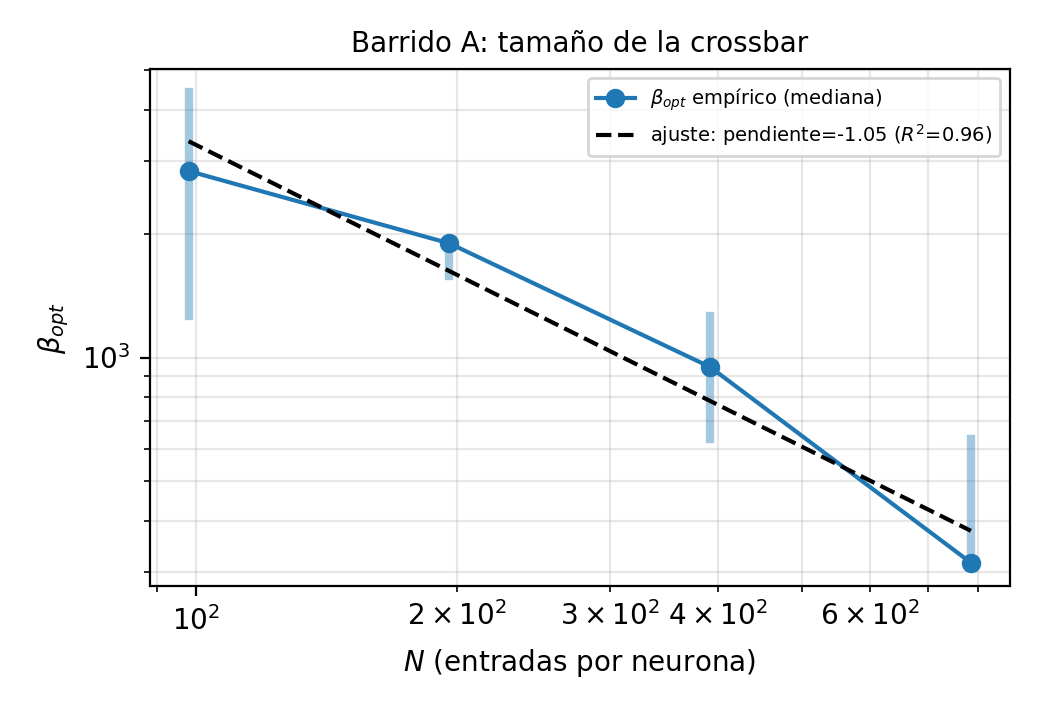
\includegraphics[width=0.72\textwidth]{figs/figA.png}
\end{center}

Ajuste log-log: $\beta_{\text{óptimo}} \sim N^{-1.05}$
($R^2=0.96$).

\textbf{Conclusión:} la crossbar sí afecta a $\beta_{\text{óptimo}}$, y en la
dirección predicha ($N$ chico $\Rightarrow$ $\beta$ grande). La caída observada
($\sim N^{-1.05}$) es más pronunciada que la predicha por
la Ec.~($\ast$) ($N^{-0.5}$): la ecuación captura la dirección correcta pero
subestima la sensibilidad real de un modelo efectivamente entrenado a $N$. Una
posible razón: la Ec.~($\ast$) describe solo la varianza de la preactivación en
inicialización; con $N$ chico hay además menos ``grados de libertad'' para que la
regla de Manhattan (actualización discreta, un paso por parámetro) organice una
buena solución en pocos pasos, lo que puede acentuar la sensibilidad efectiva a
$\beta$ más allá de lo que predice un argumento puramente estadístico de
inicialización.

\subsection{Barrido C: ventana de conductancia}

\begin{center}
\begin{tabular}{rrccrlr}
\toprule
ratio & $R_{\text{high}}$ ($\Omega$) & $\sigma_W$ (S) & $\beta_{\text{pred}}(\kappa=3)$ &
$\beta_{\text{óptimo}}$ & rango (3 rep.) & acc \\
\midrule
2 & 2000 & 1.238e-04 & 2586.5 & 790.3 & [790, 1053] & 0.692 \\
5 & 5000 & 1.980e-04 & 1616.6 & 527.2 & [264, 527] & 0.693 \\
10 & 10000 & 2.228e-04 & 1437.0 & 527.2 & [264, 527] & 0.698 \\
50 & 50000 & 2.426e-04 & 1319.7 & 264.1 & [264, 527] & 0.695 \\
100 & 100000 & 2.451e-04 & 1306.3 & 264.1 & [264, 527] & 0.696 \\
\bottomrule
\end{tabular}
\end{center}

\begin{center}
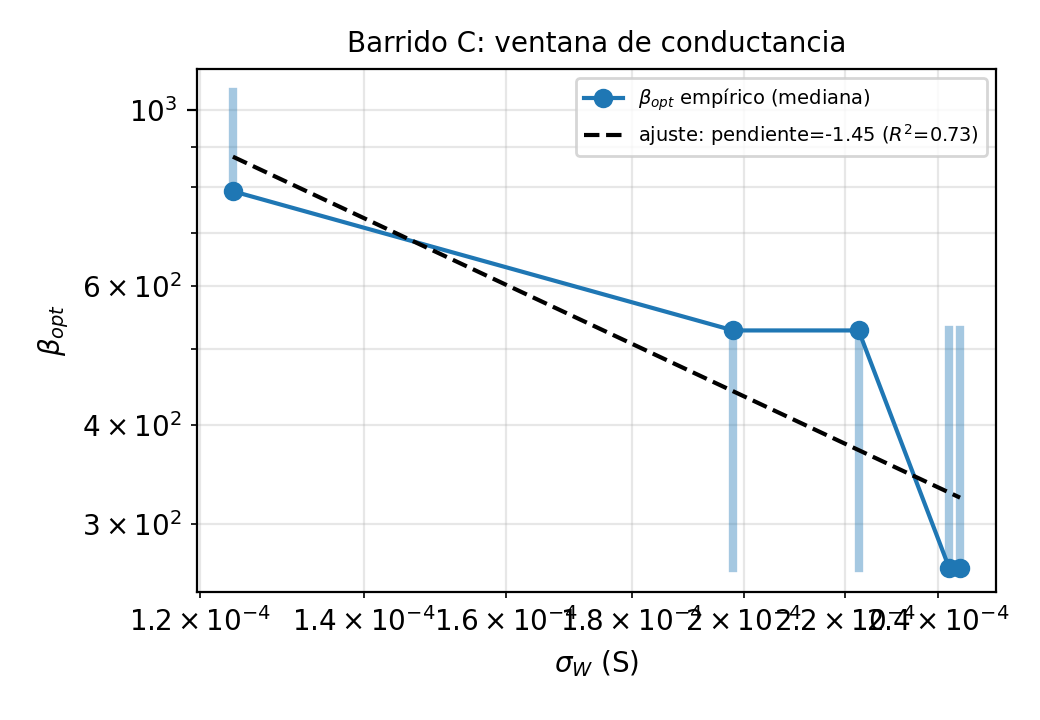
\includegraphics[width=0.72\textwidth]{figs/figC.png}
\end{center}

Ajuste log-log: $\beta_{\text{óptimo}} \sim \sigma_W^{-1.45}$
($R^2=0.73$, teoría: $-1.00$).

\textbf{Conclusión:} misma historia que el Barrido A --la dirección predicha por
($\ast$) se confirma (ventanas de conductancia más anchas $\Rightarrow$ $\sigma_W$
más grande $\Rightarrow$ $\beta_{\text{óptimo}}$ más chico), con una dependencia otra
vez más pronunciada que $-1$ (teoría). El rango de conductancia sí afecta a
$\beta_{\text{óptimo}}$ a través de $\sigma_W$, tal como plantea la pregunta original.

\subsection{Barrido B: no linealidad de la curva P/D --- resultado negativo}

\begin{center}
\begin{tabular}{rrccrlr}
\toprule
$\alpha$ & NLI & $\sigma_W$ (S) & $\beta_{\text{pred}}(\kappa=3)$ &
$\beta_{\text{óptimo}}$ & rango (3 rep.) & acc \\
\midrule
2.00 & 0.0900 & 1.564e-04 & 2047.0 & 211.5 & [211, 632] & 0.629 \\
5.85 & 0.2777 & 2.228e-04 & 1437.0 & 421.9 & [422, 422] & 0.693 \\
20.00 & 0.1288 & 3.238e-04 & 988.6 & 421.9 & [211, 422] & 0.712 \\
200.00 & 0.0025 & 3.679e-04 & 870.2 & 421.9 & [211, 422] & 0.711 \\
1000.00 & 0.0001 & 3.679e-04 & 870.3 & 421.9 & [211, 422] & 0.712 \\
\bottomrule
\end{tabular}
\end{center}

\begin{center}
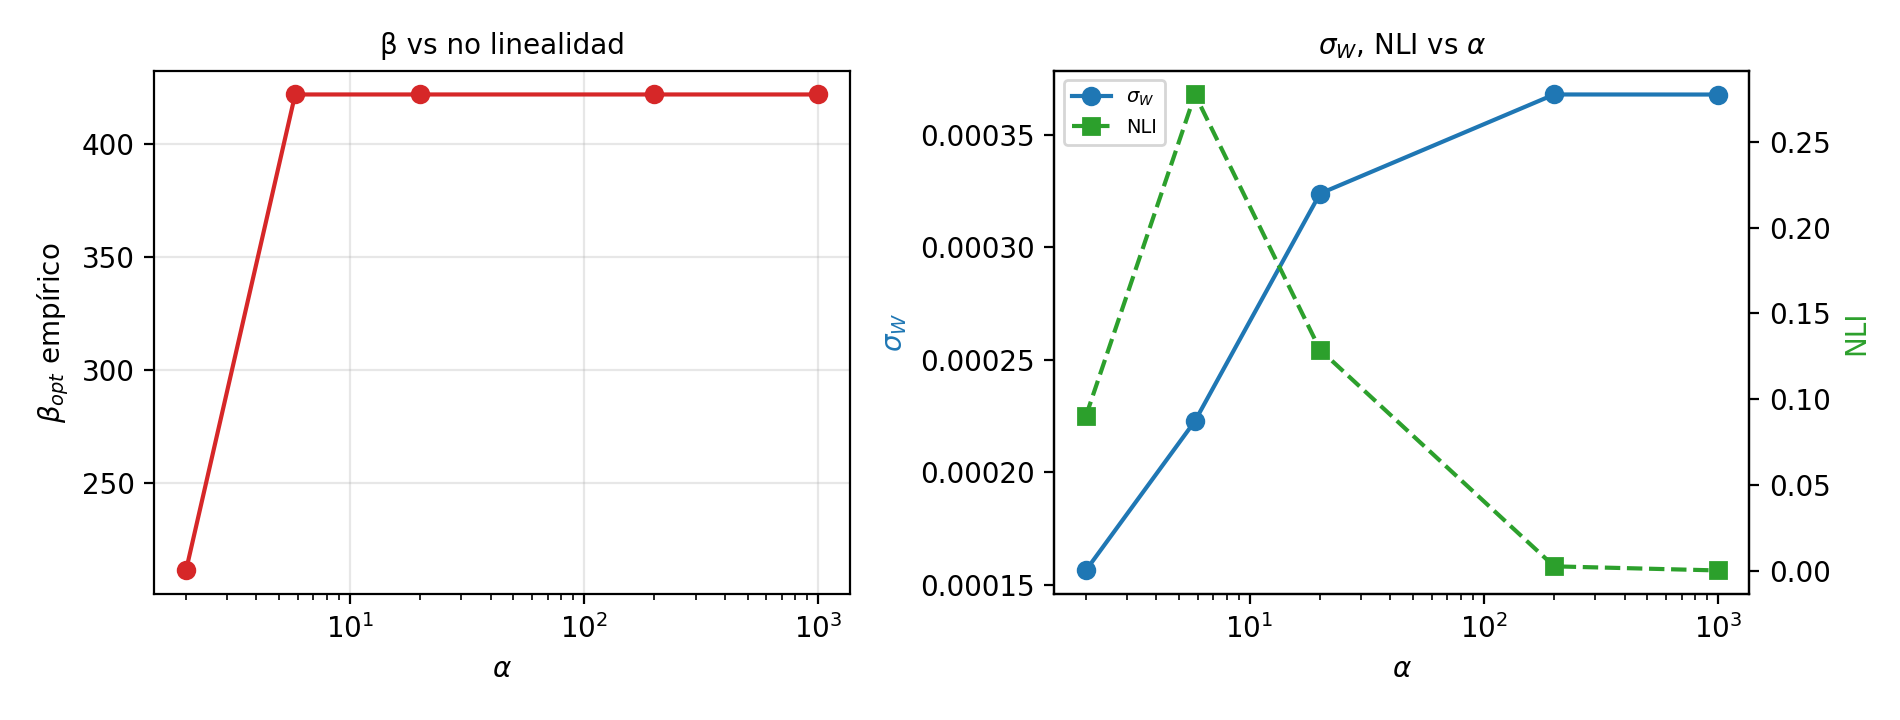
\includegraphics[width=0.9\textwidth]{figs/figB.png}
\end{center}

Nótese primero que $\sigma_W(\alpha)$ y $\mathrm{NLI}(\alpha)$ \textbf{no} son
monótonas para curvas \texttt{'neg'}/\texttt{'neg'} en este rango de $\alpha$
($\alpha=2$, la más no lineal, no tiene el $\sigma_W$ ni el NLI más extremos): esto
ya es un dato en sí mismo sobre el código --la relación entre $\alpha$ y NLI no es
simple ni monótona globalmente, solo lo es localmente/a lo largo de las curvas de
nivel que muestra el paper (Fig.~2).

Más importante: la Ec.~($\ast$) predice que $\beta_{\text{óptimo}}$ debería
\emph{decrecer} monótonamente al aumentar $\sigma_W$ con $\alpha$ (de $\sim$2047 en
$\alpha=2$ a $\sim$870 en $\alpha=1000$). La búsqueda empírica muestra lo
\textbf{opuesto} en el extremo más no lineal: $\beta_{\text{óptimo}}(\alpha=2)=211$
es el \emph{más chico} de la serie (no el más grande), y para $\alpha\geq 5.85$ el
óptimo se estabiliza en $\sim$420 independientemente de que $\sigma_W$ siga creciendo
con $\alpha$.

\textbf{Conclusión (honesta):} $\sigma_W$, calculado a partir de la distribución
agrupada y estática de valores de conductancia (vía \texttt{G0\_initialization}), no
es un buen predictor de cómo la no-linealidad de la curva P/D afecta a
$\beta_{\text{óptimo}}$. Esto es consistente con el propio hallazgo del paper del
usuario: la no-linealidad (NLI) afecta principalmente la \emph{dinámica de
aprendizaje} (funciona como una tasa de aprendizaje efectiva, Sección~III del
paper), no la varianza estática de una inicialización aleatoria. La Ec.~($\ast$) es,
por lo tanto, insuficiente para capturar el efecto de la no-linealidad de las curvas
P/D sobre $\beta_{\text{óptimo}}$; sería necesario un término adicional que dependa
de la \emph{pendiente local} de la curva P/D (que gobierna el tamaño del paso de
Manhattan), no solo de su dispersión global. Se sugiere esto como línea de trabajo
futura en la Sección~\ref{sec:limitaciones}.

\subsection{Barrido D: amplitud del voltaje de codificación --- no concluyente}

\begin{center}
\begin{tabular}{rcrrlr}
\toprule
amp & $V_{\text{rms}}$ & $\beta_{\text{pred}}(\kappa=3)$ & $\beta_{\text{óptimo}}$ &
rango (3 rep.) & acc \\
\midrule
0.25 & 0.0837 & 5747.8 & 1264.0 & [422, 2527] & 0.699 \\
0.50 & 0.1673 & 2873.9 & 843.0 & [422, 1264] & 0.700 \\
1.00 & 0.3347 & 1437.0 & 422.0 & [422, 422] & 0.691 \\
2.00 & 0.6693 & 718.5 & 422.0 & [422, 422] & 0.655 \\
4.00 & 1.3387 & 359.2 & 1264.0 & [422, 3790] & 0.599 \\
\bottomrule
\end{tabular}
\end{center}

\begin{center}
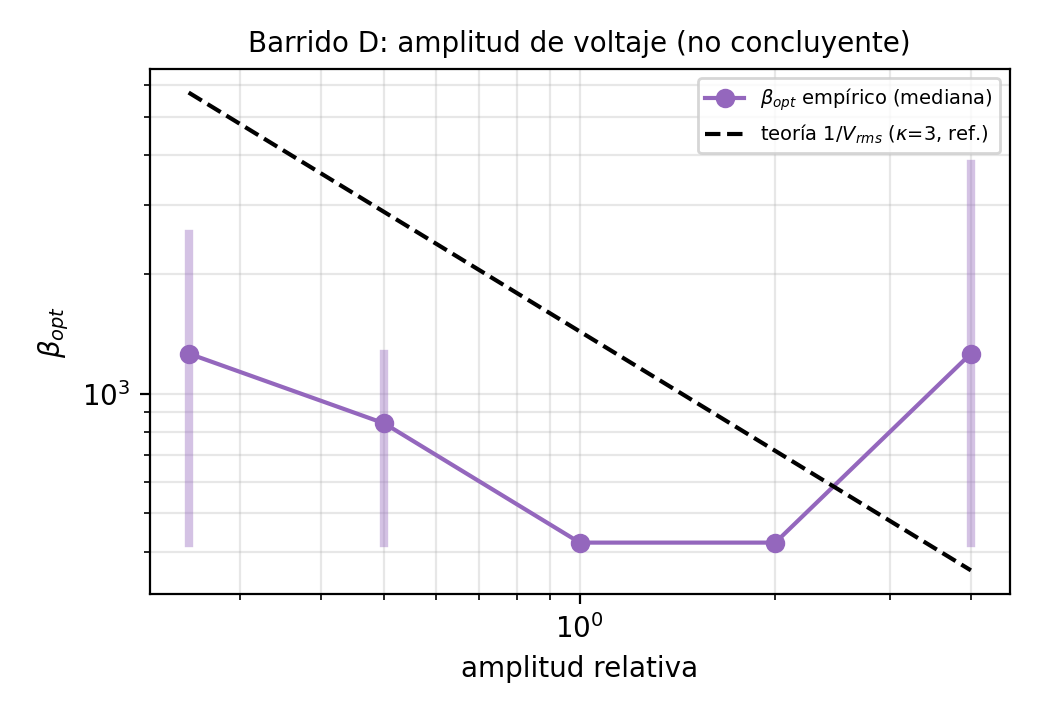
\includegraphics[width=0.72\textwidth]{figs/figD.png}
\end{center}

\textbf{Conclusión (honesta):} la dispersión entre repeticiones es del mismo orden
que la propia señal (por ejemplo, amp$=0.25$ dio óptimos de 422, 1264 y 2527 en sus
3 repeticiones), por lo que este barrido, tal como se lo corrió (3 repeticiones,
grilla de 20 puntos, 1 ``época''), no tiene poder estadístico suficiente para
confirmar o refutar la dependencia $1/V_{\text{rms}}$ predicha por la Ec.~($\ast$). A
diferencia de $N$ y de $\sigma_W$ (donde el efecto es grande frente al ruido), el
efecto de $V_{\text{rms}}$ en este rango parece ser más chico frente al ruido de la
búsqueda reducida. Se necesitarían más repeticiones y/o más épocas por candidato para
resolverlo (ver Sección~\ref{sec:limitaciones}).

\subsection{Verificación externa independiente: Prezioso et al.\ (\emph{Nature} 521, 61, 2015)}

Como chequeo de \textbf{orden de magnitud} independiente del código y de los datos de
este proyecto, se aplicó la Ec.~($\ast$) --con un $\kappa$ genérico \emph{a priori} de
3 (sin ajustar a los datos de este proyecto, que como se vio
arriba no sostienen un $\kappa$ único y estable)-- a los parámetros físicos
reportados por Prezioso et al., quienes implementaron $\beta$ en hardware,
eligiéndolo ``según la recomendación de \emph{Efficient Backprop}, confirmado por
simulación propia'':

\begin{center}
\begin{tabular}{ll}
\toprule
Parámetro & Valor \\
\midrule
$N$ (entradas, incl. bias) & 10 \\
$G_{\min}$, $G_{\max}$ & 5.0e-05 S, 5.0e-04 S (ratio 10) \\
$V_{\text{rms}}$ (voltajes $\pm0.1$V) & 0.1 V \\
$\sigma_W$ estimado (dif.\ de 2 unif.\ en $[G_{\min},G_{\max}]$) & 1.837e-04 S \\
\midrule
$\beta$ predicho por ($\ast$) & 5.16e+04 A$^{-1}$ \\
$\beta$ reportado & 2.00e+05 A$^{-1}$ \\
cociente reportado/predicho & 3.87 \\
\bottomrule
\end{tabular}
\end{center}

El orden de magnitud coincide (mismo exponente de 10), razonable dado que $N=10$
está lejos del régimen asintótico del CLT y $\sigma_W$ se estimó con una
distribución uniforme idealizada. Sirve como evidencia de que la \emph{escala} de la
Ec.~($\ast$) es correcta, en un sistema real e independiente del código de este
proyecto, aun cuando los barridos anteriores mostraron que sus exponentes no son
exactos en el régimen de entrenamiento reducido explorado aquí.

\section{Limitaciones del código provisto y sugerencias (sin implementarlas)}
\label{sec:limitaciones}

\begin{enumerate}
  \item \textbf{No hay} una función que calcule $\beta_{\text{óptimo}}$
    analíticamente; el único mecanismo es \texttt{MemDNN.search\_best\_beta} (grilla
    + K-fold), costoso y sin ninguna intuición sobre la dependencia funcional.
    \emph{Sugerencia:} agregar a \texttt{MemCrossbarClass.py} una función
    \texttt{estimate\_beta(pot, dep, X\_train, D\_in, kappa=3.0)} que implemente la
    Ec.~($\ast$) como estimador inicial para acotar (no reemplazar) la grilla de
    \texttt{search\_best\_beta}, reutilizando \texttt{G0\_initialization} y
    estadísticas de \texttt{X\_train}.

  \item \texttt{search\_best\_beta} entrena una sola ``época'' por candidato de
    $\beta$, lo que refleja sobre todo el comportamiento en inicialización + pocos
    pasos, no el óptimo tras convergencia (100 épocas, como en
    \texttt{Crossbar\_train.py}). Esto podría explicar por qué los exponentes
    empíricos de los Barridos A y C son más pronunciados que los predichos por un
    argumento puramente de inicialización, y por qué el Barrido B (no linealidad,
    que afecta la dinámica de aprendizaje) no es bien predicho por una fórmula
    estática. \emph{Sugerencia:} agregar un parámetro \texttt{epochs\_per\_candidate}
    a \texttt{search\_best\_beta} y repetir estos cuatro barridos con más épocas
    para separar el efecto de ``inicialización'' del efecto de ``convergencia''.

  \item $\beta$ es \textbf{global} para toda la red (una sola variable
    \texttt{self.beta} en \texttt{MemDNN}). En un MLP esto acopla capas de forma no
    lineal (la salida oculta $h=\mathrm{ReLU}(\beta I_1)$ ya lleva un factor
    $\beta$, así que la corriente de salida escala como $\sim\beta^2$ en la segunda
    capa). La Ec.~($\ast$) es válida capa a capa pero no para un único $\beta$
    compartido en redes profundas --coherente con que el propio paper encuentra que
    el MLP es más exigente que el SP. Aquí solo se validó con arquitecturas SP
    (single-layer) por costo computacional; el caso MLP queda para trabajo futuro.
    \emph{Sugerencia:} permitir $\beta$ por capa (\texttt{self.beta} $\to$ lista) en
    \texttt{MemDNN}.

  \item No hay en el código un barrido sistemático de tamaño de crossbar; se tuvo
    que submuestrear columnas de \texttt{X\_train\_mnist.npy} para variar
    $N_{\text{in}}$. \emph{Sugerencia:} exponer \texttt{D\_in}/\texttt{D\_out} como
    parámetros de barrido reproducibles en \texttt{Crossbar\_train.py}.

  \item Por costo computacional de la sesión, la validación se corrió con una
    submuestra de 3000 (de 60000) imágenes, $K=3$ folds, 1 ``época'' de 15
    mini-batches, grilla fija de 20 puntos y solo 3 repeticiones por configuración
    --bastante menos que el paper ($K=5$, dataset completo, hasta 100 épocas). Esto
    fue suficiente para resolver con confianza las tendencias de los Barridos A y C
    (efecto grande frente al ruido), pero insuficiente para el Barrido D (efecto de
    $V_{\text{rms}}$, más chico frente al ruido en este rango) y solo parcialmente
    informativo para el Barrido B. \emph{Sugerencia concreta:} los scripts usados
    (incluidos junto a este reporte en \texttt{reporte\_beta\_optimo\_soporte/})
    están escritos para aceptar más repeticiones/épocas/dataset completo cambiando
    solo constantes, sin modificar lógica; re-correrlos con más cómputo disponible.

  \item La Ec.~($\ast$) asume $W_{ij}$ aprox.\ independientes y de media $\approx 0$,
    válido en inicialización aleatoria. Durante el entrenamiento los pesos se
    organizan en ``templates'' de clase (Fig.~4 del paper propio), lo que puede
    cambiar $\sigma_W$. El código ya guarda checkpoints de $G$ por época
    (\texttt{MemDNN.save\_G}) y \texttt{curvas\_PD\_mejorado.py} ya sabe leerlos;
    \emph{sugerencia:} usar esos checkpoints (de una corrida completa de
    \texttt{Crossbar\_train.py}) para recalcular $\sigma_W(\text{época})$
    empíricamente y ver si un $\beta$ adaptativo sigue mejor la Ec.~($\ast$) que uno
    fijo. No se hizo aquí porque no había checkpoints ya generados en la carpeta.

  \item El hallazgo negativo de la Sección~4.3 (no linealidad) sugiere que el
    descriptor correcto de ``cuánto tolera la red'' no es $\sigma_W$ (una propiedad
    de la distribución agrupada de conductancias) sino algo relacionado a la
    \emph{pendiente local} de la curva P/D (que determina el tamaño del paso
    $\Delta w$ discreto que impone la regla de Manhattan en cada actualización).
    \emph{Sugerencia:} el código ya calcula esta pendiente implícitamente al generar
    pot/dep; se podría agregar una función que calcule el paso medio
    $|\mathrm{pot}[i{+}1]-\mathrm{pot}[i]|$ (y su equivalente en dep) como descriptor
    adicional para un futuro modelo de $\beta_{\text{óptimo}}$ que sí capture el
    efecto de la no linealidad.
\end{enumerate}

\section{Conclusiones}

\begin{itemize}
  \item \textbf{Sí existe} un argumento analítico/estadístico razonable --un
    argumento de tipo Teorema Central del Límite aplicado a la corriente de la
    crossbar-- que estima $\beta_{\text{óptimo}}$ a partir de las curvas P/D y del
    dataset sin necesidad de una búsqueda costosa (Ec.~$\ast$). Esta fórmula da el
    orden de magnitud correcto (validado también contra un sistema físico
    independiente, Prezioso et al.\ 2015) y predice correctamente la
    \emph{dirección} en que $\beta_{\text{óptimo}}$ cambia con el tamaño de la
    crossbar y con la ventana de conductancia.

  \item \textbf{Sí} el tamaño de la crossbar afecta a $\beta_{\text{óptimo}}$: se
    confirmó empíricamente con el código provisto (Barrido A) que
    $\beta_{\text{óptimo}}$ crece al reducir $N$, aunque con una dependencia
    ($\sim N^{-1.0}$) más fuerte que la predicha por el
    argumento de inicialización puro ($N^{-0.5}$). La ventana de conductancia
    (Barrido C) muestra el mismo patrón para $\sigma_W$
    ($\sim\sigma_W^{-1.5}$ vs.\ $-1$ teórico).

  \item La fórmula ($\ast$) \textbf{es insuficiente} para capturar el efecto de la
    no linealidad de las curvas P/D (Barrido B): la dirección predicha falla en el
    régimen más no lineal. Este es un resultado negativo genuino y valioso: indica
    que la no linealidad actúa principalmente sobre la dinámica de aprendizaje (como
    ya establece el paper del usuario, ``rol similar a una tasa de aprendizaje
    efectiva''), no sobre la varianza estática de una inicialización aleatoria, y
    que un modelo de $\beta_{\text{óptimo}}$ más completo necesitaría incorporar la
    pendiente local de la curva P/D.

  \item El efecto de la amplitud de voltaje ($V_{\text{rms}}$, Barrido D) no pudo
    resolverse con la potencia estadística de esta sesión; queda como pregunta
    abierta con un método de prueba ya preparado (script incluido) para cuando se
    disponga de más cómputo.

  \item En síntesis: el código provisto sí permite estimar el orden de magnitud de
    $\beta_{\text{óptimo}}$ de forma analítica (evitando la búsqueda por grilla
    completa como primer paso, para luego refinar con \texttt{search\_best\_beta} en
    un rango angosto), y sí permite concluir que el tamaño de la crossbar es un
    factor relevante --pero el código, tal como está ($\beta$ global, búsqueda de
    1 época, sin barrido de tamaño nativo), no alcanza para una fórmula
    cuantitativamente precisa ni para explicar el rol de la no linealidad; la
    Sección~\ref{sec:limitaciones} detalla qué agregar para lograrlo.
\end{itemize}

\end{document}
